% !TEX root = ../main.tex
\ulfgchapter{3}{Simulator, Radar Specification and Dataset Design}{chp:simulator}

\section{Introduction}

Chapter~\ref{chp:background} described detection in general terms. This chapter specifies the
particular radar, the particular simulator and the particular datasets that every result in this
report is measured on. All the numeric values deliberately withheld from Chapter~\ref{chp:background}
are introduced here.

Three decisions in this chapter shape everything that follows.

The first is the choice to work in simulation. It is what makes a controlled comparison possible at
all, because it supplies exact ground truth and independent control over each difficulty. It is
also the reason Chapter~\ref{chp:realdata} exists, since a result obtained entirely inside a
simulator says nothing on its own about real measurements.

The second is the sensor specification. The radar is matched to the range--Doppler bin geometry of
the real dataset used later, so a target occupies a comparable number of cells in both domains.
Without that, any transfer failure in Chapter~\ref{chp:realdata} could be dismissed as a resolution
mismatch rather than a finding. Section~\ref{sec:carrada_spec} records how those parameters were
derived, including why the bandwidth published by the dataset's own authors was not used.

The third is the dataset design. The benchmark is stratified rather than randomly sampled, so that
the conditions in which CFAR is documented to fail are present in measurable quantity rather than
appearing by chance.

\section{Why simulate}

A comparison of the kind attempted here needs three things that measured radar data does not
readily provide.

\textbf{Exact ground truth.} Scoring $\Pd$ requires knowing precisely which cells contain targets.
Real datasets provide annotations, which are themselves estimates, produced semi-automatically and
carrying their own error. In simulation the target position is an input, not an inference.

\textbf{Independent control of difficulty.} The failure modes of
Section~\ref{sec:cfar_failures} --- clutter edges, target masking --- must be produced deliberately
and in isolation to be measured separately. In recorded data they co-occur uncontrollably.

\textbf{Sufficient quantity in rare conditions.} The conditions that discriminate between detectors
are exactly the ones that are rare in naturally sampled data.

The cost is external validity, and it is a real cost. A detector tuned inside one simulator may
have learned that simulator rather than radar. This is why the synthetic benchmark of
Chapter~\ref{chp:synthetic} is treated in this report as an internally valid measurement whose
generalisation is a separate question, tested in Chapter~\ref{chp:realdata} and not assumed here.

\section{Radar specification}
\label{sec:carrada_spec}

\subsection{Matching the real dataset's bin geometry}

The sensor parameters were chosen so that a target occupies the same number of range and Doppler
cells in simulation as in CARRADA~\cite{ouaknine2021carrada}, the real dataset used in
Chapter~\ref{chp:realdata}. Detectors operate in bins: a CFAR window is a fixed number of cells
wide, and a network's receptive field is a fixed number of cells across. If a target spread over
three cells in one domain and eight in the other, a transfer failure would be a trivial scaling
artefact rather than evidence about the detector.

Table~\ref{tab:bingeom} shows the match achieved.

\begin{table}[H]
\centering
\caption{Range--Doppler bin geometry: the real dataset and the simulator used here.}
\label{tab:bingeom}
\begin{tabular}{@{}lcc@{}}
\toprule
 & \textbf{CARRADA} & \textbf{Simulator} \\
\midrule
Map size (range $\times$ Doppler) & $256 \times 64$ & $\RadarRangeBins \times \RadarM$ \\
Range span & \SI{0}{\metre}--\SI{50}{\metre} & \SI{0}{\metre}--\SI{\RadarRangeMax}{\metre} \\
Range per bin & \SI{0.195}{\metre} & \SI{\RadarRangeRes}{\metre} \\
Velocity span & $\pm\SI{13.43}{\metre\per\second}$ &
$\pm\SI{\RadarVelMax}{\metre\per\second}$ \\
Velocity per bin & \SI{0.42}{\metre\per\second} &
\SI{\RadarVelRes}{\metre\per\second} \\
Frame time & \SI{4.635}{\milli\second} & \SI{\RadarFrameTime}{\milli\second} \\
\bottomrule
\end{tabular}
\end{table}

\subsection{The published parameter table is internally inconsistent}

Matching those bins was not a matter of copying the dataset's published parameters, because those
parameters do not agree with each other. CARRADA's parameter table quotes a sweep bandwidth of
\SI{\CarradaQuotedB}{\giga\hertz} alongside a range resolution of \SI{0.20}{\metre}, a maximum
range of \SI{50}{\metre} and 256 range bins. These cannot all hold simultaneously, and the
discrepancy matters here because bandwidth is what sets range resolution.

Four checks establish which of the published values are reliable.

\textbf{The stated formula contradicts the stated number.} The paper gives the standard relation
$\Delta R = c/2B$. Substituting \SI{4}{\giga\hertz} yields \SI{0.0375}{\metre}, against the
\SI{0.20}{\metre} printed in the same table --- a factor of more than five.

\textbf{The angle entry reveals what the table means by ``resolution''.} The same table quotes an
angular resolution of \ang{0.70}. The physical resolution of the array described is on the order of
\ang{14}. But \ang{180} divided by 256 angle bins is \ang{0.703}. The entries labelled
``FFT resolution'' are therefore \emph{bin spacings}, not physical resolutions.

\textbf{Applying that reading to the range axis is self-consistent.} \SI{50}{\metre} over 256 range
bins gives \SI{\CarradaBinSpacing}{\metre} per bin, which is the \SI{0.20}{\metre} printed.

\textbf{A genuine \SI{4}{\giga\hertz} sampled sweep would make the dataset impossible.} With 256
samples per chirp at that bandwidth, the maximum unambiguous range would be about
\SI{9.6}{\metre}. The dataset's own figures describe objects at \SI{8}{\metre} and
\SI{33}{\metre}, so the \SI{50}{\metre} span is real and the \SI{4}{\giga\hertz} is not the
bandwidth that produced these bins.

The most likely reading is that \SI{4}{\giga\hertz} is the configured radio-frequency sweep of the
front end, of which only the portion falling inside the sampled beat band contributes to the range
transform. Reproducing the observed bin spacing over the observed span requires an effective
bandwidth of
\begin{equation}
B_{\text{eff}} = \frac{c \, N_{\text{bins}}}{2 R_{\max}} \approx \SI{\CarradaBeff}{\mega\hertz},
\end{equation}
which is the value adopted here, rounded to \SI{\RadarB}{\mega\hertz}.

The velocity axis, by contrast, is fully self-consistent: the quoted velocity resolution implies a
frame time of \SI{4.635}{\milli\second}, which divided by 64 chirps gives a chirp duration of
\SI{\RadarTc}{\micro\second}, and that in turn reproduces the quoted maximum velocity to within
\SI{0.01}{\metre\per\second}. That agreement is a useful cross-check that the rest of the table is
trustworthy and only the bandwidth entry is anomalous.

\subsection{Resulting parameters}

Table~\ref{tab:radarspec} lists the specification adopted. These values are read directly from the
simulator's configuration when this report is built, so the two cannot drift apart.

\begin{table}[H]
\centering
\caption{Sensor specification and the quantities derived from it.}
\label{tab:radarspec}
\begin{tabular}{@{}llr@{}}
\toprule
\textbf{Quantity} & \textbf{Symbol or formula} & \textbf{Value} \\
\midrule
Carrier frequency & $f_c$ & \SI{\RadarFc}{\giga\hertz} \\
Sweep bandwidth & $B$ & \SI{\RadarB}{\mega\hertz} \\
Chirp duration & $T_c$ & \SI{\RadarTc}{\micro\second} \\
Samples per chirp & $N$ & \RadarN{} \\
Chirps per frame & $M$ & \RadarM{} \\
\midrule
Wavelength & $c/f_c$ & \SI{\RadarLambda}{\milli\metre} \\
Chirp slope & $B/T_c$ & \SI{\RadarSlope}{\mega\hertz\per\micro\second} \\
Sampling frequency & $N/T_c$ & \SI{\RadarFs}{\mega\hertz} \\
Range resolution & $c/2B$ & \SI{\RadarRangeRes}{\metre} \\
Maximum range & $c f_s / 4S$ & \SI{\RadarRangeMax}{\metre} \\
Velocity resolution & $\lambda/2MT_r$ & \SI{\RadarVelRes}{\metre\per\second} \\
Maximum velocity & $\pm\lambda/4T_r$ & \SI{\RadarVelMax}{\metre\per\second} \\
Frame time & $M T_r$ & \SI{\RadarFrameTime}{\milli\second} \\
\midrule
Coherent processing gain & $10\log_{10}(NM)$ & \SI{\RadarCoherentGain}{\deci\bel} \\
Processing gain after windowing & measured & \SI{\RadarProcGain}{\deci\bel} \\
\bottomrule
\end{tabular}
\end{table}

Two consequences are worth recording. The maximum range is set by the Nyquist limit of the sampled
beat band: a target at \SI{\RadarRangeMax}{\metre} produces a beat frequency of exactly $f_s/2$.
And the processing gain falls from the coherent \SI{\RadarCoherentGain}{\deci\bel} to
\SI{\RadarProcGain}{\deci\bel} once window functions are applied. That second figure is the one
that matters for difficulty calibration, and it is derived analytically from the window functions
rather than assumed, so it tracks any change to the configuration.

\section{The simulator}

\subsection{Signal generation and processing}

The simulator reproduces the processing chain described in Chapter~\ref{chp:background} rather than
approximating its output. For each frame it synthesises the transmitted chirp, forms each target's echo as a
delayed and attenuated copy, sums the echoes, mixes the result with the transmitted signal to
obtain the beat signal, and applies the two Fourier transforms. The range--Doppler map is therefore
produced by the same operations as in a real receiver, and effects such as spectral leakage,
scalloping loss and the finite mainlobe width arise naturally instead of being modelled.

Figure~\ref{fig:simchain} shows the additions that turn this chain into a benchmark generator.

\begin{figure}[H]
\centering
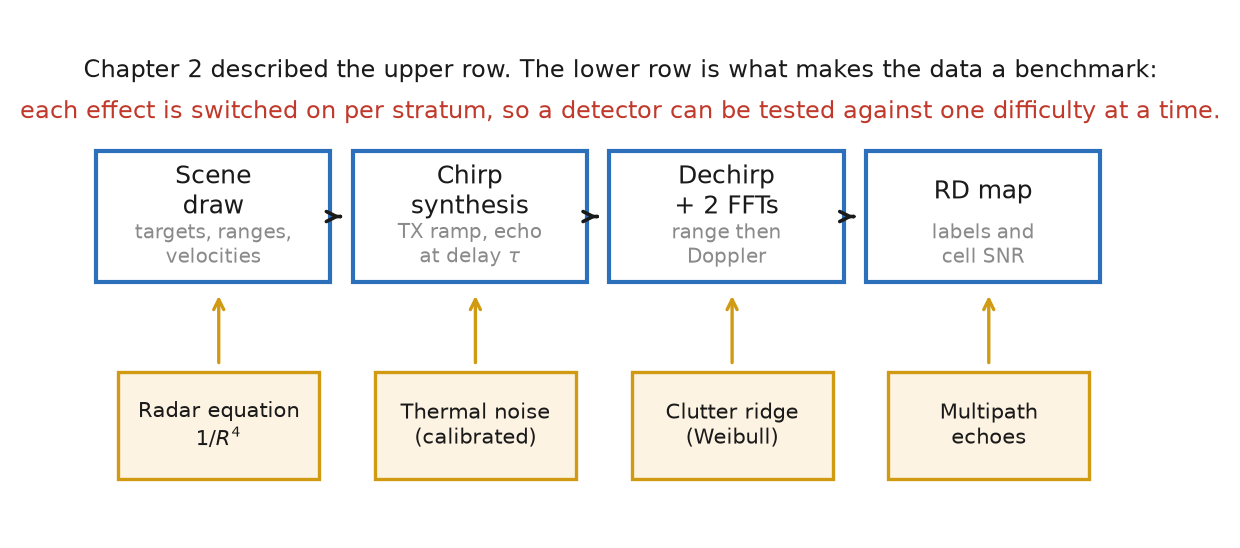
\includegraphics[width=\textwidth]{figures/Chapter3/ch3_fig1_simulator_chain.png}
\caption[Simulator structure]{The upper row is the processing chain of
Chapter~\ref{chp:background}. The lower row is what makes the output a benchmark: each effect can
be enabled independently per stratum, so a detector can be tested against one difficulty at a
time.}
\label{fig:simchain}
\end{figure}

\subsection{Propagation, clutter and multipath}

\textbf{Propagation.} Received power follows the radar equation, falling as $1/R^4$. This is
enabled in every stratum so that the physics is consistent across the benchmark, referenced to
\SI{25}{\metre}. The consequence is that range and difficulty are coupled: a distant target is
genuinely harder, as it is in practice.

\textbf{Clutter.} The zero-Doppler ridge is modelled as a band of elevated return around zero
velocity, with a Weibull texture rather than a Gaussian one. The shape parameter is swept, lower
values giving spikier clutter, so that the rate at which each detector degrades as clutter becomes
heavier-tailed is measurable rather than assumed. Its strength is specified as a clutter-to-noise
ratio, which keeps it meaningful when the noise level changes.

\textbf{Multipath.} A delayed, attenuated echo is optionally added, producing a secondary response
offset in range from the true target.

\section{Difficulty calibration}

\subsection{What signal-to-noise ratio means here}

Difficulty must be specified in a way that means the same thing to every detector, and that is less
straightforward than it appears. An SNR defined on the raw received samples is not the quantity a
detector experiences, because the two Fourier transforms concentrate a target's energy into one
cell while spreading noise across all of them. That coherent gain is
\SI{\RadarProcGain}{\deci\bel} for this configuration, so a target specified at
\SI{-10}{\deci\bel} on the raw samples arrives at the detector some \SI{30}{\deci\bel} above the
noise floor and is trivially detectable.

Difficulty is therefore specified as \emph{cell SNR at the detector}: the ratio of a target's peak
cell power to the noise power in a cell of the finished range--Doppler map. The noise variance
required to realise a requested cell SNR is computed analytically from the configuration, and the
achieved value is then \emph{measured per target} and stored alongside the label. The stored value,
not the requested one, is used in every analysis, so scalloping loss and propagation are accounted
for rather than ignored.

\subsection{Where the difficulty sits}

Figure~\ref{fig:snrdist} shows the resulting distribution across the test split.

\begin{figure}[H]
\centering
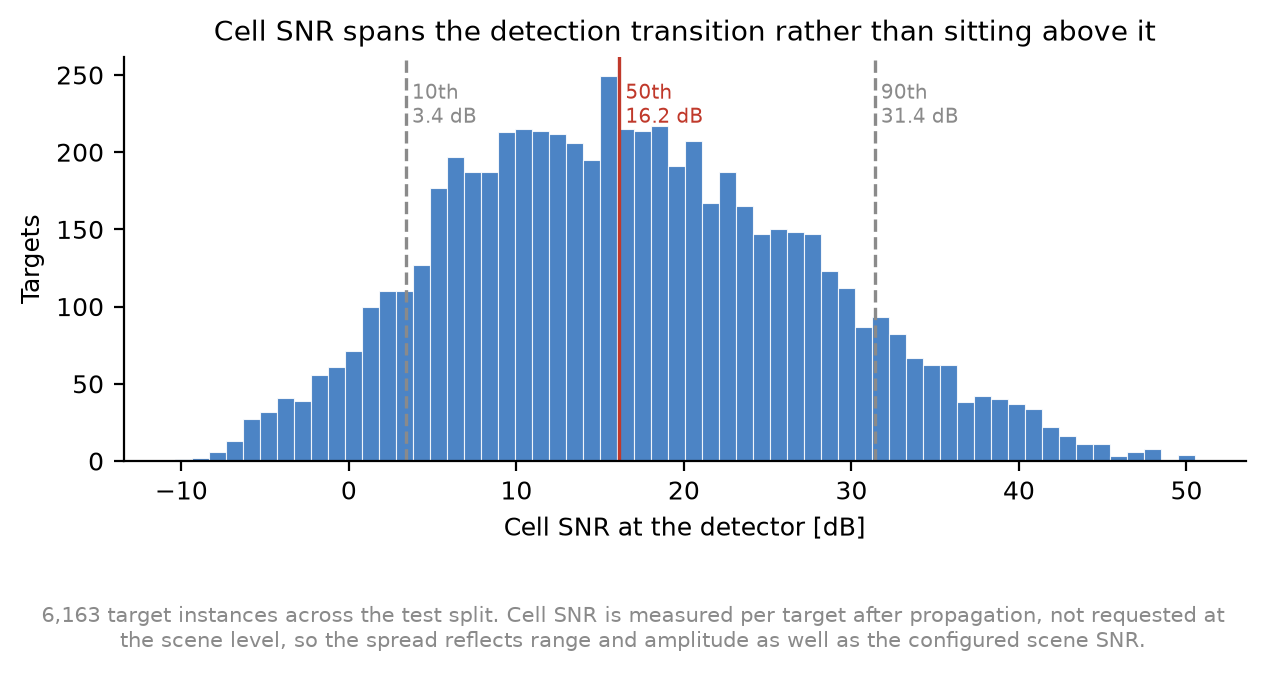
\includegraphics[width=0.92\textwidth]{figures/Chapter3/ch3_fig4_snr_distribution.png}
\caption[Cell SNR distribution]{Measured cell SNR for every target in the test split. The spread
reflects range and target amplitude as well as the configured scene SNR, because propagation is
applied before the measurement.}
\label{fig:snrdist}
\end{figure}

The spread is deliberate. A benchmark concentrated well above the detection threshold would be
solved by every method and would discriminate between none of them; one concentrated below it would
be solved by none. An earlier configuration sat about \SI{2}{\deci\bel} lower, which placed a
fifth of all targets below \SI{5}{\deci\bel} cell SNR --- undetectable by any method --- and
bunched the clutter strata near $\Pd \approx 0.15$, where detectors cannot be told apart. The scene
level was raised accordingly.

\section{Dataset design}

\subsection{Why stratified rather than randomly sampled}

The conditions that separate detectors are rare under random sampling. An earlier randomly sampled
dataset produced target masking in \SI{1.1}{\percent} of frames and unresolvable pairs in
\SI{0.4}{\percent}, and measured performance tracked that coverage almost monotonically --- which
means the headline number was largely a statement about the sampling, not about the detectors.

The benchmark is therefore stratified: each condition is generated in equal quantity, and results
are reported per stratum rather than pooled. This gives a reliable estimate within each condition,
and it makes the composition of the benchmark an explicit design choice rather than an accident.

\subsection{The eight strata}

Table~\ref{tab:strata} lists them, and Figure~\ref{fig:strata} shows one frame from each.

\begin{table}[H]
\centering
\caption{The eight strata. Each is generated in equal quantity. Seven contain targets and are
scored; \texttt{noise} contains none and supports false-alarm measurement.}
\label{tab:strata}
\begin{tabular}{@{}p{2.4cm}p{6.2cm}p{4.3cm}@{}}
\toprule
\textbf{Stratum} & \textbf{Content} & \textbf{Purpose} \\
\midrule
\texttt{isolated} & One target, homogeneous noise & Control: the condition where CA-CFAR is
close to optimal \\
\addlinespace
\texttt{masking} & Strong and weak pair, separation swept across the resolution limit &
The masking failure mode of Section~\ref{sec:cfar_failures} \\
\addlinespace
\texttt{clutter} & Target inside the zero-Doppler ridge & Detection against heavy-tailed clutter \\
\addlinespace
\texttt{clutter\_edge} & Target in clean noise, with the CFAR window reaching into the ridge &
The clutter-edge failure mode. Also the condition in which a published CNN
\emph{loses}~\cite{yavuz2021radcnn} \\
\addlinespace
\texttt{multi} & Four to five targets, all pairs beyond the window reach & Dense scenes without
masking \\
\addlinespace
\texttt{noise} & Empty frames & False-alarm measurement and threshold calibration \\
\addlinespace
\texttt{mixed} & Variable target count, clutter and multipath together & A realistic combination
rather than one isolated effect \\
\addlinespace
\texttt{unresolved} & Pair inside a single mainlobe & Physics cap: no detector can separate them,
so it acts as a sanity check \\
\bottomrule
\end{tabular}
\end{table}

\begin{figure}[H]
\centering
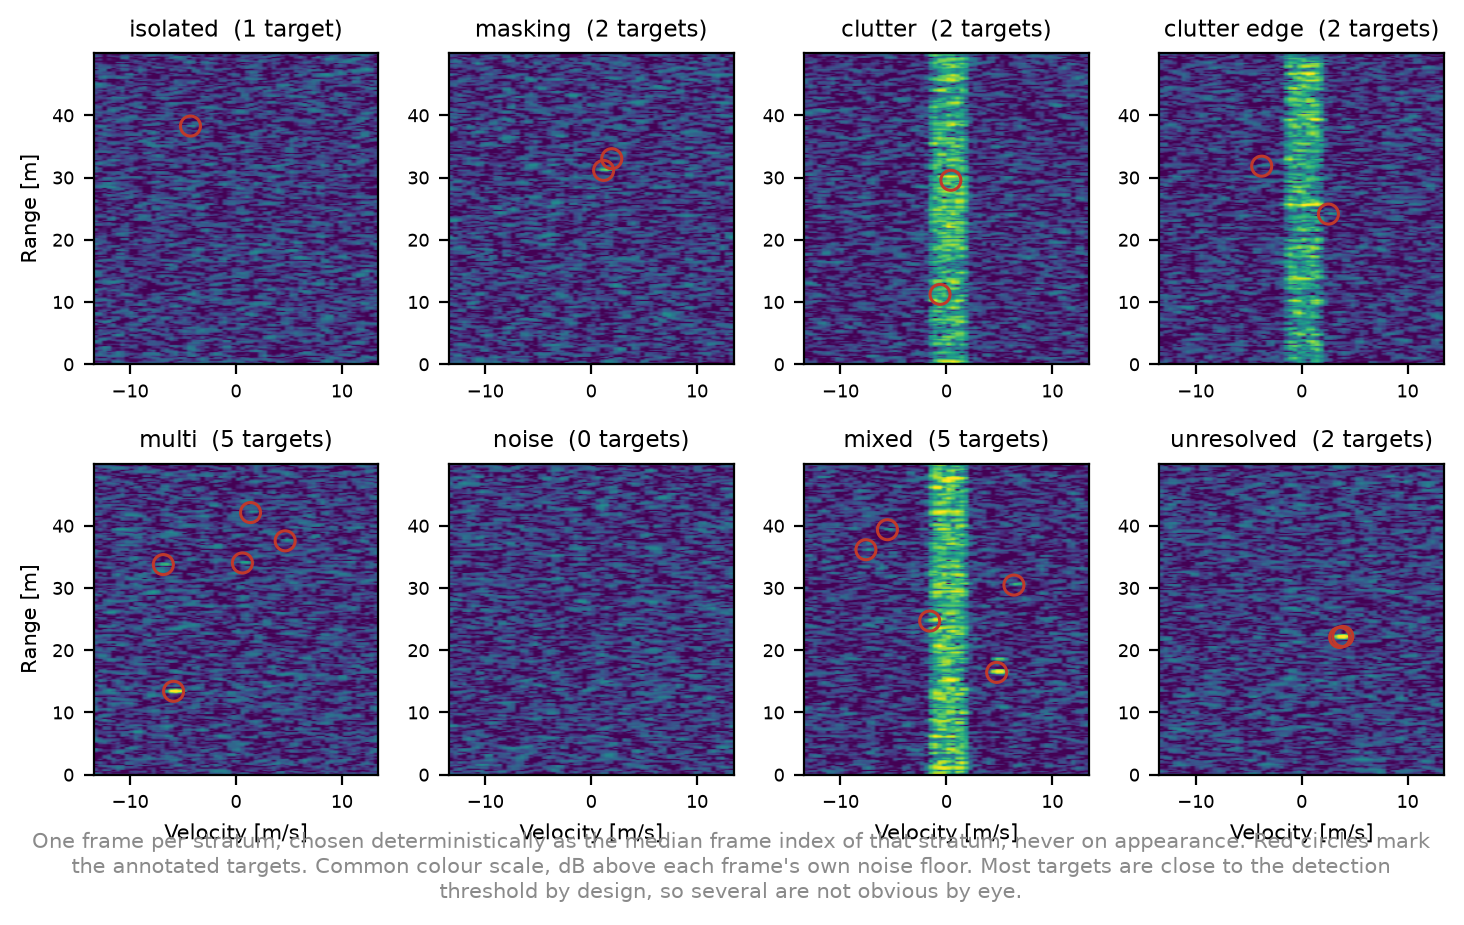
\includegraphics[width=\textwidth]{figures/Chapter3/ch3_fig2_strata_montage.png}
\caption[The eight strata]{One frame from each stratum, selected deterministically as the median
frame index of that stratum rather than by appearance. Red circles mark the annotated targets.
Several are not obvious by eye, which is by design: the benchmark places targets near the detection
transition.}
\label{fig:strata}
\end{figure}

Two design points in that table are worth drawing out.

The \texttt{clutter\_edge} stratum exists specifically because the literature review of
Section~\ref{sec:sota} identified it as the condition where a published learned detector loses. A
benchmark that omitted it would be systematically flattering. Its velocity band was set by
measurement rather than by the nominal ridge width: the Doppler window smears the ridge well past
its nominal edge, still \SI{13.6}{\deci\bel} above the floor at \SI{1.68}{\metre\per\second}, so a
lower bound at the nominal edge would have placed a third of these targets inside the clutter
skirt and merely duplicated the \texttt{clutter} stratum.

The \texttt{unresolved} stratum cannot be won by any detector, and is retained deliberately. A
method reporting high $\Pd$ there would indicate a fault in the evaluation rather than a capable
detector, and this stratum is what exposed one such fault during development.

\subsection{Splits}

Five datasets are generated from the same configuration with different random seeds.

\begin{table}[H]
\centering
\caption{Dataset splits. Frame counts are read from the generated data when this report is built.}
\label{tab:splits}
\begin{tabular}{@{}llr@{}}
\toprule
\textbf{Split} & \textbf{Role} & \textbf{Frames} \\
\midrule
\texttt{bench2\_train} & Network training & \BenchTrainFrames \\
\texttt{bench2\_val} & Threshold selection, epoch selection & \BenchValFrames \\
\texttt{bench2\_tune} & CFAR window geometry selection & \BenchTuneFrames \\
\texttt{bench2\_test} & The reported numbers. Read once & \BenchTestFrames \\
\texttt{bench2\_snr\_sweep} & Detection probability against cell SNR & \BenchSnrSweepFrames \\
\bottomrule
\end{tabular}
\end{table}

The separation of \texttt{tune} from \texttt{val} is deliberate. The CFAR window geometry and the
network's operating point are both selected quantities, and selecting them on the same data that
sets the other arm's threshold would introduce exactly the asymmetry
Section~\ref{sec:problem} identified. Chapter~\ref{chp:detectors} describes both selections.

\section{Verification}

A simulator is an instrument, and an instrument that has not been checked cannot support a
measurement. Three checks were run before any detector result was produced.

\textbf{Point spread function.} An isolated target was placed and its response measured along both
axes, on-bin and deliberately off-bin. Figure~\ref{fig:psf} shows the result. The mainlobe spans
approximately two bins, which is what fixes the guard-cell count of the CFAR window in
Chapter~\ref{chp:detectors}: the guard region must cover a target's own spread, or a target would
inflate its own threshold.

\begin{figure}[H]
\centering
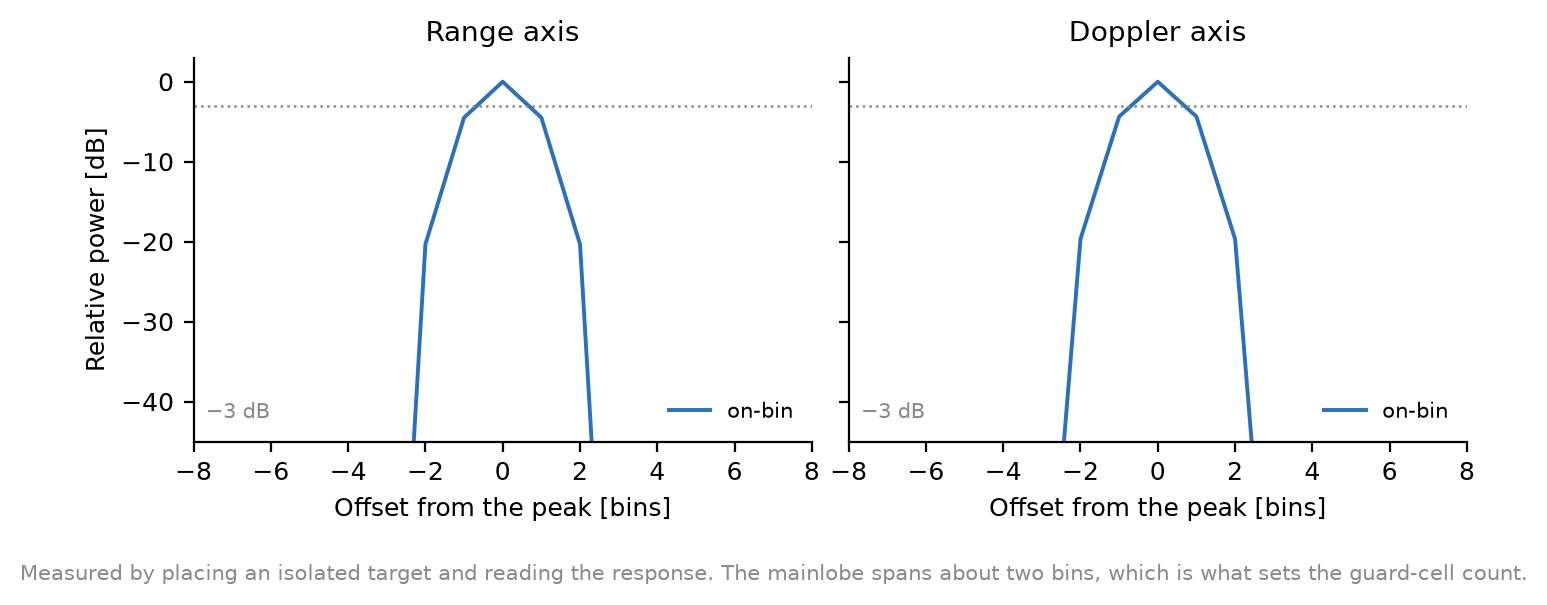
\includegraphics[width=\textwidth]{figures/Chapter3/ch3_fig3_psf.png}
\caption[Measured point spread function]{Response of an isolated target along each axis, measured
rather than assumed. The off-bin case shows the loss incurred when a target does not fall at a bin
centre.}
\label{fig:psf}
\end{figure}

\textbf{Resolution limits.} Measured on the same data, two equal-strength targets require about
\SI{0.39}{\metre} of range separation to appear as separate peaks, rising to \SI{0.59}{\metre} when
one partner is weak, and \SI{1.16}{\metre\per\second} in Doppler. These measurements set the
separation ranges swept in the \texttt{masking} and \texttt{unresolved} strata, so that both sit
across the real limit rather than at an assumed one.

\textbf{Label alignment.} Every generated target was checked against the peak actually present in
the map. Alignment is exact above about \SI{22}{\deci\bel} cell SNR. Below that a small fraction of
labels do not coincide with the strongest local peak; this was investigated and traced to noise
spikes exceeding a weak target, which is a property of the physics rather than a labelling fault,
and it disappears at high SNR as a genuine bug would not.

\section{Conclusion}

This chapter specified the instrument. The radar reproduces the range--Doppler bin geometry of the
real dataset used in Chapter~\ref{chp:realdata}, using an effective bandwidth of
\SI{\RadarB}{\mega\hertz} derived from that dataset's own bin spacing rather than from its
published and internally inconsistent bandwidth figure. The simulator generates frames through the
full signal chain, with propagation, clutter and multipath switchable per stratum. Difficulty is
specified as measured cell SNR at the detector, not as a scene-level quantity, and the resulting
distribution spans the detection transition.

The benchmark is stratified into eight equal conditions chosen to include both the regime where
CA-CFAR is close to optimal and the regimes where it is documented to fail, including one condition
selected specifically because a published learned detector loses there. Five splits separate
training, threshold selection, window selection, the SNR sweep and the single scored test set.

Chapter~\ref{chp:detectors} now specifies the two detectors that operate on these frames, and
fixes the evaluation protocol before any comparative result is produced.
